\begin{frame}{Closed-Set Accuracy Predicts Open-Set Performance}
  \begin{columns}[T,onlytextwidth]
    \column{0.58\textwidth}
      \begin{itemize}\scriptsize\itemsep0.3em
        \item \textbf{Finding} (Vaze et al., ICLR 2022): on standard open-set benchmarks, AUROC grows almost linearly with closed-set accuracy, Pearson $\rho = 0.95$ across MSP, ARPL (Adversarial Reciprocal Point Learning) and ARPL+CS (ARPL with generated confusing samples).
        \item \textbf{ImageNet scale:} across CNN, ViT and MLP-Mixer (all-MLP) classifiers, $\rho = 0.88$ on the Hard unknown split and $0.63$ on the Easy one (next slide); within ResNets, $0.99$ and $1.00$. ViT-B/16 lies above the trend, but its ImageNet-21K pre-training contains the ``unknown'' classes.
        \item \textbf{Proposed reason:} cross-entropy is a proper scoring rule (optimal at the true probabilities), so lower test error should bring better calibration (confidence matching accuracy), and low confidence then flags a new class more reliably.
        \item \textbf{Recipe:} longer training, stronger augmentation, label smoothing, then MLS scoring (both earlier in this lecture). TinyImageNet AUROC: 57.7 for the published MSP baseline, 83.0 for MLS; ARPL+CS: 78.2 published, 82.5 retrained. Over six benchmarks MLS gains 15.6 points on average, 0.03 from the retrained ARPL+CS.
      \end{itemize}
    \column{0.40\textwidth}
      \centering
      \vspace{0.4em}
      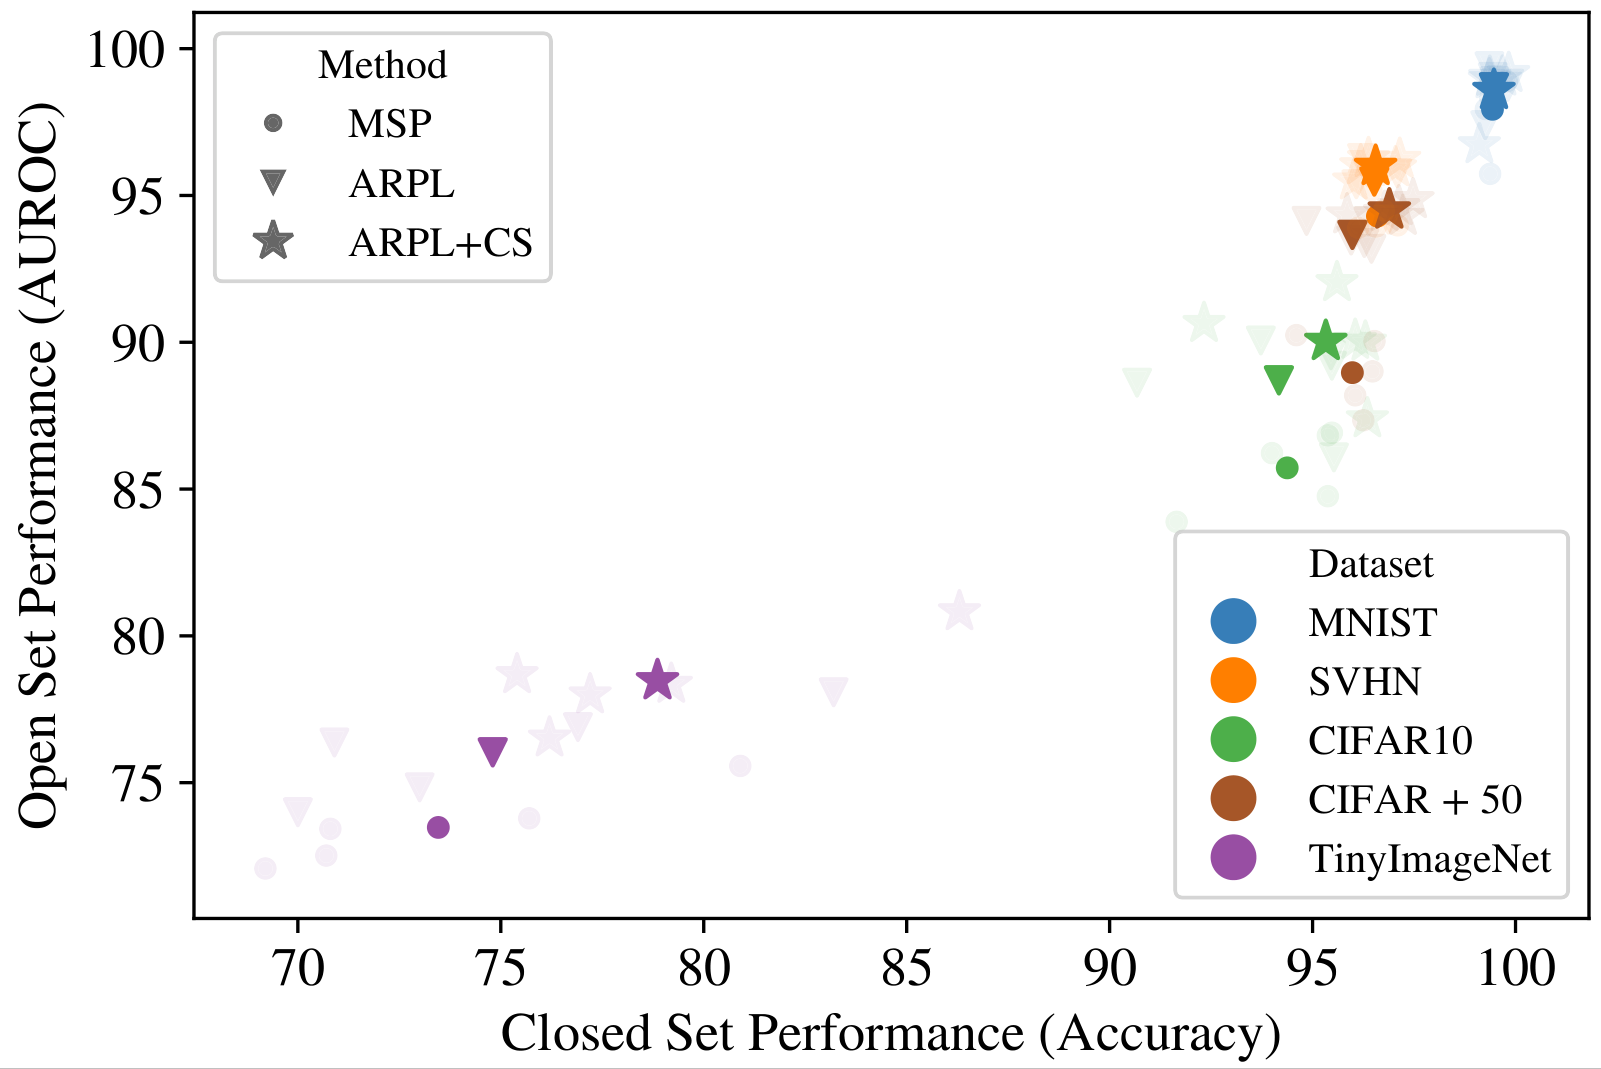
\includegraphics[width=\linewidth,height=0.56\textheight,keepaspectratio]{images/image-recognition/osr_fig2_closed_vs_open_set_correlation.png}\\[0.2em]
      {\scriptsize Bold markers: mean over five known/unknown class splits; faint markers: single splits. Vaze et al., ``Open-Set Recognition: a Good Closed-Set Classifier is All You Need?'' ICLR 2022, \href{https://arxiv.org/abs/2110.06207v2}{arXiv:2110.06207v2}, Figure~2.\par}
  \end{columns}
\end{frame}

\begin{frame}{The Semantic Shift Benchmark}
  \centering
  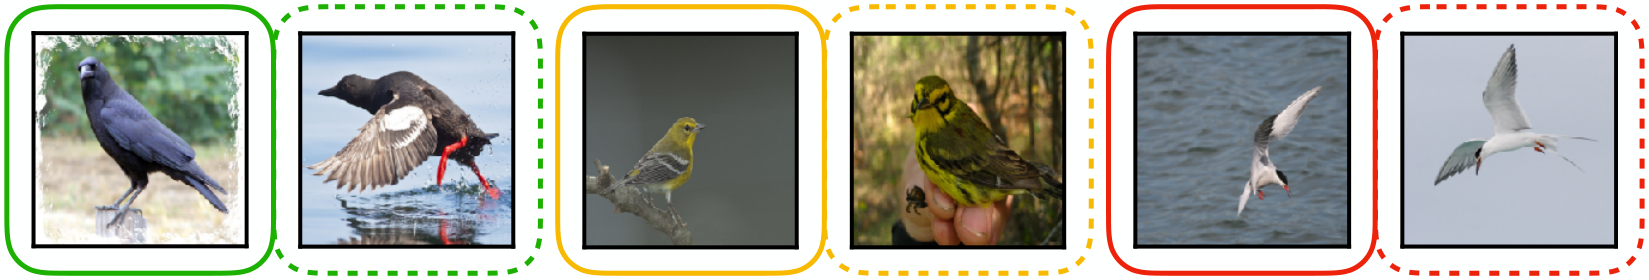
\includegraphics[width=\textwidth,height=0.30\textheight,keepaspectratio]{images/image-recognition/osr_fig5_cub_open_set_class_pairs.png}\\[0.1em]
  {\scriptsize Unknown CUB class (dashed) next to its closest known class (solid); green, orange, red: Easy, Medium, Hard. Vaze et al., \href{https://arxiv.org/abs/2110.06207v2}{arXiv:2110.06207v2}, Figure~5.\par}
  \vspace{0.3em}
  \begin{columns}[T,onlytextwidth]
    \column{0.52\textwidth}
      \begin{itemize}\scriptsize\itemsep0.25em
        \item \textbf{Semantic Shift Benchmark (SSB):} unknown classes of CUB, Stanford Cars and FGVC-Aircraft (earlier in this lecture) are binned Easy, Medium or Hard by attribute similarity to the known classes (CUB: 312 attributes, e.g.\ \texttt{has\_bill\_shape::hooked}).
        \item \textbf{ImageNet:} the 1K classes are known; ImageNet-21K-P classes sorted by summed hierarchy distance to them form 1,000-class Easy and Hard sets.
        \item Old splits (6 known, 4 unknown CIFAR-10 classes) leave novelty undefined. Hard costs MLS 5.9 AUROC points on ImageNet; 10$\times$ more random unknowns cost about 0.6.
      \end{itemize}
    \column{0.46\textwidth}
      \centering
      {\scriptsize
      \setlength{\tabcolsep}{3.5pt}
      \begin{tabular}{lcccc}
        \toprule
         & \textbf{Known} & \textbf{Closed} & \multicolumn{2}{c}{\textbf{AUROC}} \\
        \cmidrule(lr){4-5}
        \textbf{Dataset} & \textbf{classes} & \textbf{acc.} & \textbf{Easy} & \textbf{Hard} \\
        \midrule
        CUB & 100 & 86.2 & 88.3 & 79.3 \\
        Stanford Cars & 98 & 97.1 & 94.0 & 82.2 \\
        FGVC-Aircraft & 50 & 91.7 & 90.7 & 82.3 \\
        ImageNet & 1000 & 78.8 & 78.7 & 72.8 \\
        \bottomrule
      \end{tabular}\par}
      \vspace{0.3em}
      {\scriptsize ResNet-50 scored with MLS; Hard includes the Medium bin where one exists. Vaze et al., \href{https://arxiv.org/abs/2110.06207v2}{arXiv:2110.06207v2}, Tables~2--3.\par}
  \end{columns}
\end{frame}

\begin{frame}{OpenOOD v1.5: Near-OOD Versus Far-OOD}
  \begin{columns}[T,onlytextwidth]
    \column{0.58\textwidth}
      \begin{itemize}\scriptsize\itemsep0.3em
        \item \textbf{Setup} (Zhang et al., DMLR 2024): ImageNet-1K is the in-distribution (ID) set. Near-OOD: SSB-hard (980 classes from SSB's 1,000-class Hard ImageNet split) and NINCO (5,879 hand-curated images). Far-OOD: iNaturalist, Textures, OpenImage-O. Nearly 40 methods, tuned on held-out validation sets.
        \item \textbf{Near-OOD stays hard:} with a ResNet-50, ASH gets 95.74 AUROC on far-OOD but 78.17 on near-OOD (MSP: 85.23 and 76.02); near-OOD gains trail far-OOD gains (right).
        \item \textbf{No single winner:} ReAct and ASH lead on ImageNet but are less competitive on CIFAR. AugMix training (mixed augmented copies of each image) plus ASH gives the best near-OOD AUROC, 82.16.
        \item \textbf{Backbones:} ViT-B/16 and Swin-T detect OOD no better than ResNet-50, despite higher top-1 accuracy (81.1\% and 81.6\% vs 76.2\%). A DINOv2 linear probe beats a supervised ViT-B on every OOD split; zero-shot CLIP helps mainly on far-OOD.
        \item \textbf{Full-spectrum test:} adding covariate-shifted ID images (ImageNet-C corruptions, -R, -V2) costs most methods over 10 near-OOD AUROC points: detectors also reject shifted images of known classes.
      \end{itemize}
    \column{0.40\textwidth}
      \centering
      \vspace{0.6em}
      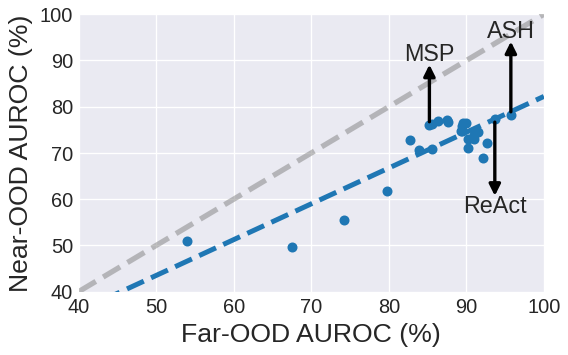
\includegraphics[width=\linewidth,height=0.50\textheight,keepaspectratio]{images/image-recognition/openood_fig2_near_vs_far_ood_auroc.png}\\[0.2em]
      {\scriptsize One dot per method on ImageNet-1K with a ResNet-50; grey dashes: equal near- and far-OOD AUROC; blue dashes: fitted trend. Zhang et al., ``OpenOOD v1.5: Enhanced Benchmark for Out-of-Distribution Detection,'' DMLR 2024, \href{https://arxiv.org/abs/2306.09301v5}{arXiv:2306.09301v5}, Figure~2.\par}
  \end{columns}
\end{frame}

\begin{frame}{Zero-Shot OOD Detection with CLIP: MCM}
  \begin{columns}[T,onlytextwidth]
    \column{0.50\textwidth}
      \begin{itemize}\scriptsize\itemsep0.3em
        \item \textbf{Zero-shot OOD detection:} only the $K$ ID class names are given, no ID images. MCM (Maximum Concept Matching; Ming et al., NeurIPS 2022) scores an image $x$ with CLIP (covered earlier):
          \[ S_{\mathrm{MCM}}(x) = \max_{i} \frac{e^{s_i(x)/\tau}}{\sum_{j=1}^{K} e^{s_j(x)/\tau}} \]
          $s_i(x)$: cosine between the image embedding of $x$ and the text embedding of ``this is a photo of a $\langle y_i \rangle$''; $\tau$: temperature (1 in the paper). Reject $x$ if $S_{\mathrm{MCM}}(x) < \lambda$, with $\lambda$ passing 95\% of ID images.
      \end{itemize}
    \column{0.48\textwidth}
      \begin{itemize}\scriptsize\itemsep0.3em
        \item \textbf{Role of the softmax:} OOD images have near-equal cosines to all ID labels, and with many classes an ID image's top cosine is only slightly higher; a softmax with moderate $\tau$ widens the gap (provably, above a threshold $\tau$, under this near-uniformity).
        \item \textbf{Temperature} (below): FPR95 is 40.75\% without softmax, 31.85\% at $\tau = 0.01$ (CLIP's smallest training temperature), 18.13\% at $\tau = 1$; the predicted class is unchanged. ImageNet-1K, ViT-B/16: AUROC 90.77, FPR95 42.74 (raw maximum cosine: 83.59, 69.08).
      \end{itemize}
  \end{columns}
  \vspace{0.1em}
  \centering
  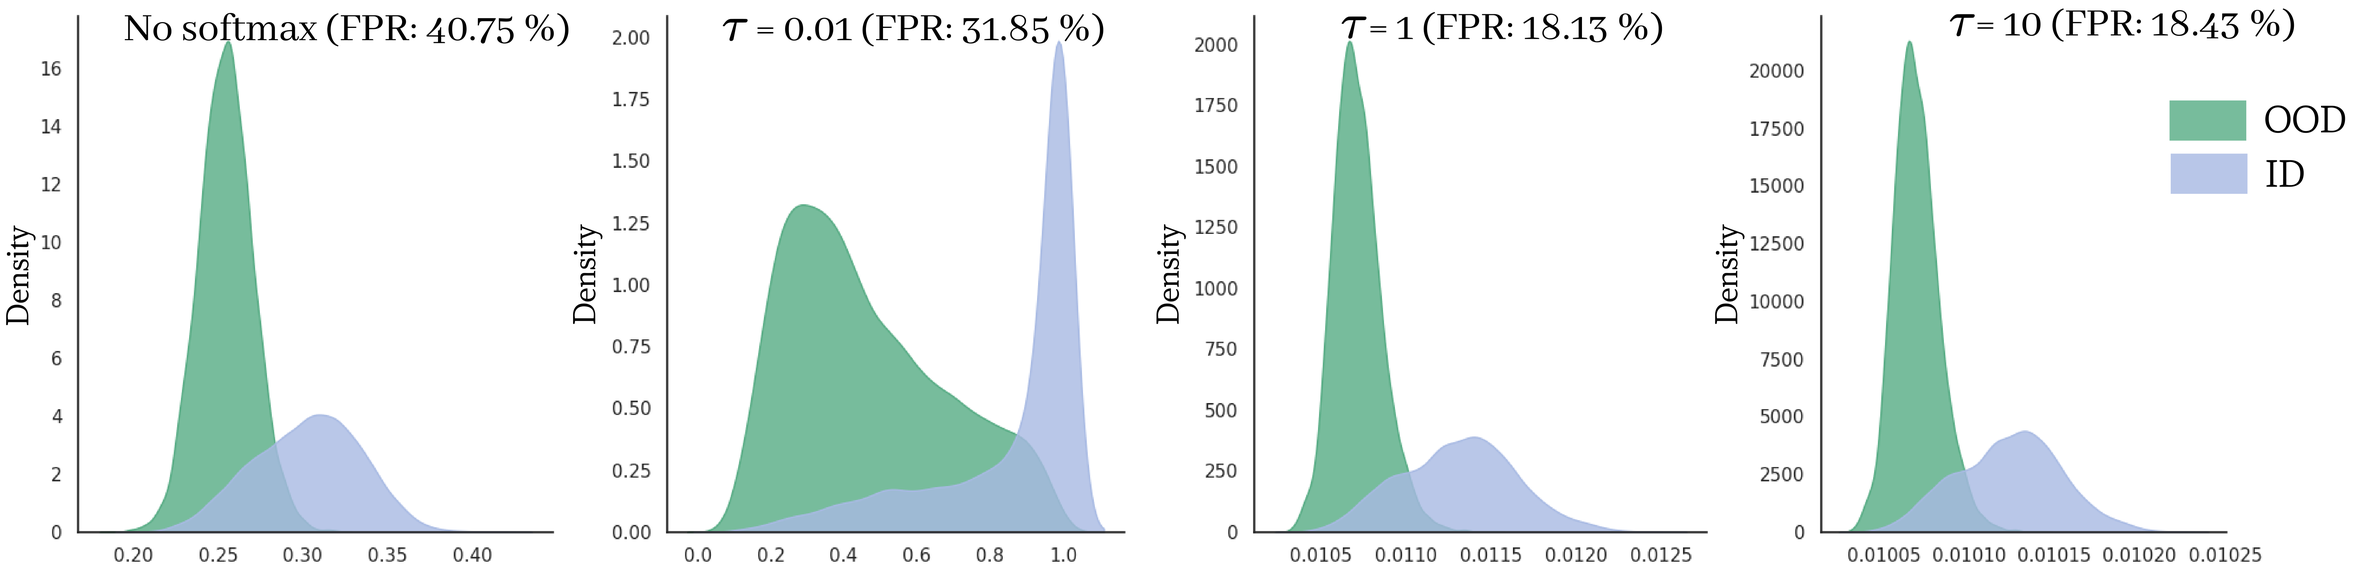
\includegraphics[width=\textwidth,height=0.30\textheight,keepaspectratio]{images/image-recognition/mcm_fig4_softmax_temperature.png}\\[0.1em]
  {\scriptsize ImageNet-100 as ID, iNaturalist as OOD. Ming et al., ``Delving into Out-of-Distribution Detection with Vision-Language Representations,'' NeurIPS 2022, \href{https://arxiv.org/abs/2211.13445v1}{arXiv:2211.13445v1}, Figure~4.\par}
\end{frame}

\begin{frame}{NegLabel: Scoring Against Negative Labels}
  \begin{columns}[T,onlytextwidth]
    \column{0.54\textwidth}
      \begin{itemize}\scriptsize\itemsep0.3em
        \item \textbf{Idea} (Jiang et al., ICLR 2024): MCM compares an image only with the $K$ ID labels. NegLabel adds $M = 10{,}000$ negative labels, nouns and adjectives from the WordNet lexical database whose text embeddings are far from every ID label; OOD images match some of them more closely than ID images do.
        \item \textbf{NegMining:} rank candidate words by the 5th percentile of their negative cosine similarities to the ID labels (a minimum that tolerates outlier labels) and keep the top $M$.
        \item \textbf{Score:}
          \[ S(x) = \frac{\sum_{i=1}^{K} e^{c_i/\tau}}{\sum_{i=1}^{K} e^{c_i/\tau} + \sum_{j=1}^{M} e^{\tilde{c}_j/\tau}} \]
          $c_i$, $\tilde{c}_j$: cosine similarity of the image embedding of $x$ with ID label $i$ and negative label $j$; $\tau = 0.01$. The sum over ID labels tolerates confusions between ID classes (husky vs malamute); averaging over 100 groups of negatives limits chance matches.
        \item \textbf{Cost:} about 1\,ms per image at $M = 10{,}000$; ID predictions are unchanged.
      \end{itemize}
    \column{0.44\textwidth}
      \centering
      {\scriptsize
      \setlength{\tabcolsep}{4pt}
      \begin{tabular}{llcc}
        \toprule
        \textbf{Method} & \textbf{Training} & \textbf{AUROC}\,$\uparrow$ & \textbf{FPR95}\,$\downarrow$ \\
        \midrule
        MSP & fine-tuned & 81.63 & 69.61 \\
        Energy & fine-tuned & 91.54 & 39.89 \\
        $k$-NN & fine-tuned & 90.97 & 42.19 \\
        \addlinespace[0.15em]
        MCM (re-run) & none & 90.82 & 43.93 \\
        NegLabel & none & 94.21 & 25.40 \\
        \bottomrule
      \end{tabular}\par}
      \vspace{0.2em}
      {\scriptsize ImageNet-1K as ID, CLIP ViT-B/16 (fine-tuned on ImageNet-1K where marked), mean of four OOD sets; MCM as re-run by Jiang et al. Jiang et al., ``Negative Label Guided OOD Detection with Pretrained Vision-Language Models,'' ICLR 2024, \href{https://arxiv.org/abs/2403.20078v1}{arXiv:2403.20078v1}, Table~1.\par}
      \begin{itemize}\scriptsize
        \item \textbf{LoCoOp} (Miyai et al., NeurIPS 2023) trains CoOp prompts (earlier in this lecture) on a few labelled images and pushes patch features whose top-200 classes miss the true label, mostly background, toward uniform ID predictions. 16-shot AUROC with MCM: 92.69 (CoOp: 91.93).
      \end{itemize}
  \end{columns}
\end{frame}

\begin{frame}{Generalized Category Discovery: GCD and SimGCD}
  \begin{columns}[T,onlytextwidth]
    \column{0.52\textwidth}
      \begin{itemize}\scriptsize\itemsep0.3em
        \item \textbf{Setting} (GCD: Generalized Category Discovery; Vaze et al., CVPR 2022): labelled images $\mathcal{D}_L$ of classes $\mathcal{Y}_L$, unlabelled images $\mathcal{D}_U$ of classes $\mathcal{Y}_U \supset \mathcal{Y}_L$; every image in $\mathcal{D}_U$ gets an old class or a new cluster.
        \item \textbf{GCD:} fine-tune a DINO ViT-B/16 (covered earlier) with SupCon (earlier in this lecture) on $\mathcal{D}_L$ plus self-supervised contrastive learning on all images, then run $k$-means with each labelled image fixed to its class's cluster.
        \item \textbf{Metric:} clustering accuracy (ACC), the fraction of $\mathcal{D}_U$ labelled correctly under the best one-to-one cluster-to-class map, found once by the Hungarian algorithm (an exact solver for one-to-one assignment); reported on All, Old ($\mathcal{Y}_L$) and New classes.
        \item \textbf{SimGCD} (Wen et al., ICCV 2023): cosine prototypes on backbone features, trained toward the sharpened prediction of another view (self-distillation); $-\varepsilon H(\bar{\mathbf{p}})$, the weighted entropy of the batch-mean prediction $\bar{\mathbf{p}}$, counters the bias toward Old classes. CUB inference: 18\,s vs 9\,min for $k$-means.
      \end{itemize}
    \column{0.46\textwidth}
      \centering
      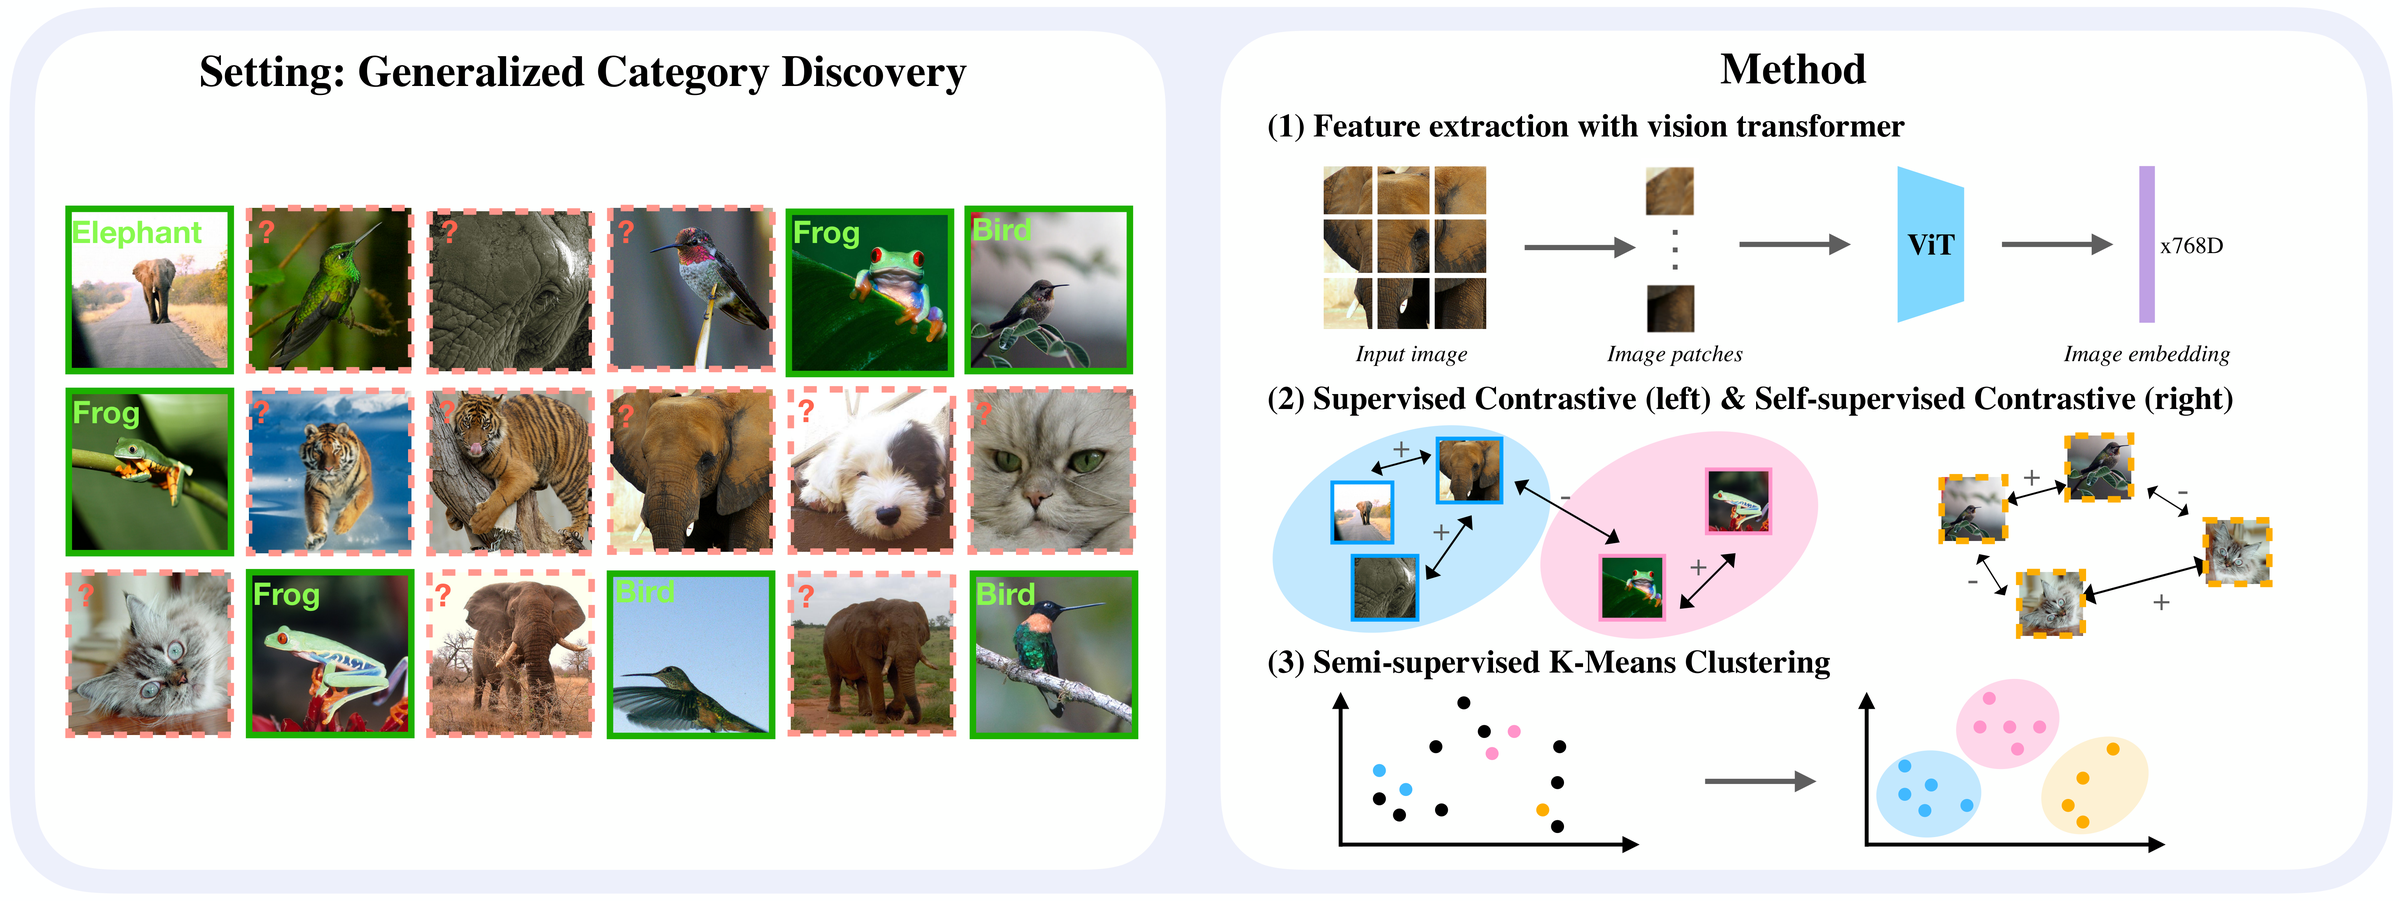
\includegraphics[width=\linewidth,height=0.30\textheight,keepaspectratio]{images/image-recognition/gcd_fig1_setting_and_method.png}\\[0.1em]
      {\scriptsize Vaze et al., ``Generalized Category Discovery,'' CVPR 2022, \href{https://arxiv.org/abs/2201.02609v2}{arXiv:2201.02609v2}, Figure~1.\par}
      \vspace{0.4em}
      {\scriptsize
      \setlength{\tabcolsep}{3.5pt}
      \begin{tabular}{lcccc}
        \toprule
         & \multicolumn{2}{c}{\textbf{GCD}} & \multicolumn{2}{c}{\textbf{SimGCD}} \\
        \cmidrule(lr){2-3}\cmidrule(lr){4-5}
        \textbf{ACC (\%)} & All & New & All & New \\
        \midrule
        CUB & 51.3 & 48.7 & 60.3 & 57.7 \\
        Stanford Cars & 39.0 & 29.9 & 53.8 & 45.0 \\
        FGVC-Aircraft & 45.0 & 46.9 & 54.2 & 51.8 \\
        \bottomrule
      \end{tabular}\par}
      \vspace{0.2em}
      {\scriptsize SSB splits; $k$-means on raw DINO features: 34.3 All on CUB. Wen et al., ``Parametric Classification for Generalized Category Discovery: A Baseline Study,'' ICCV 2023, \href{https://arxiv.org/abs/2211.11727v4}{arXiv:2211.11727v4}, Tables~2 and~5.\par}
  \end{columns}
\end{frame}

\begin{frame}{An Open-World Recognition Loop in Practice}
  \begin{columns}[T,onlytextwidth]
    \column{0.50\textwidth}
      \centering
      \vspace{0.3em}
      \resizebox{\linewidth}{!}{%
      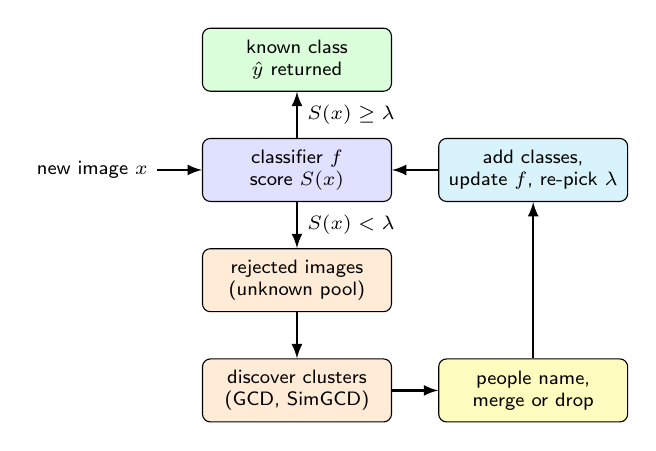
\begin{tikzpicture}[font=\sffamily\scriptsize, >=latex,
          box/.style={draw, rounded corners=0.1cm, align=center, minimum width=2.4cm, minimum height=0.8cm},
          arr/.style={->, thick}]
        \node (x) at (0,3.2) {new image $x$};
        \node[box, fill=blue!12] (f) at (2.6,3.2) {classifier $f$\\score $S(x)$};
        \node[box, fill=green!14] (acc) at (2.6,4.6) {known class\\$\hat{y}$ returned};
        \node[box, fill=orange!16] (pool) at (2.6,1.8) {rejected images\\(unknown pool)};
        \node[box, fill=orange!16] (disc) at (2.6,0.4) {discover clusters\\(GCD, SimGCD)};
        \node[box, fill=yellow!25] (name) at (5.6,0.4) {people name,\\merge or drop};
        \node[box, fill=cyan!15] (upd) at (5.6,3.2) {add classes,\\update $f$, re-pick $\lambda$};
        \draw[arr] (x) -- (f);
        \draw[arr] (f) -- node[right] {$S(x) \geq \lambda$} (acc);
        \draw[arr] (f) -- node[right] {$S(x) < \lambda$} (pool);
        \draw[arr] (pool) -- (disc);
        \draw[arr] (disc) -- (name);
        \draw[arr] (name) -- (upd);
        \draw[arr] (upd) -- (f);
      \end{tikzpicture}}\\[0.4em]
      {\scriptsize Adapted from Bendale and Boult, ``Towards Open World Recognition,'' CVPR 2015, \href{https://arxiv.org/abs/1412.5687v1}{arXiv:1412.5687v1}, Figure~1, with a discovery step added before labelling.\par}
    \column{0.48\textwidth}
      \begin{itemize}\scriptsize\itemsep0.4em
        \item \textbf{Open-world recognition} (Bendale and Boult, CVPR 2015): detect unknowns, collect them, have people label them, then learn the new classes incrementally. Category discovery reduces the labelling to naming clusters.
        \item \textbf{Threshold:} pick $\lambda$ on held-out ID images for a target TPR (e.g.\ 95\%), using validation data only, and re-pick it after every update of $f$, since the score distribution moves with the model.
        \item \textbf{Monitor the rejection rate:} at 95\% TPR, about 5\% of ID images are rejected by design. A sustained rise signals new classes or covariate shift; inspect samples first, because detectors also reject shifted images of known classes.
        \item \textbf{Before adding classes:} wait for stable clusters, estimate how many there are (GCD's estimate for CUB: 231 against 200 true classes), and re-test old classes on a fixed audit set after each update.
      \end{itemize}
  \end{columns}
\end{frame}
